\documentclass[11pt]{article}

% ---------- Packages ----------
\usepackage[a4paper,margin=1in]{geometry}
\usepackage{graphicx}
\usepackage{microtype}
\usepackage{amsmath,amssymb}
\usepackage{placeins}
\usepackage{booktabs}
\usepackage{fontawesome5}
\usepackage{hyperref}
\usepackage{caption}
\usepackage{subcaption}
\usepackage[superscript]{cite}
\usepackage{array}

\usepackage{setspace}
\onehalfspacing

% TikZ for the pipeline figure
\usepackage{tikz}
\usetikzlibrary{arrows.meta,positioning}

% ---------- Metadata ----------
\title{Alignment-Free Detection of Horizontal Gene Transfer Candidates\\
via Protein Similarity Graphs and Anomaly Scoring}

\author{}
\date{}

\begin{document}
\maketitle
\vspace{-52pt}

\begin{center}
\renewcommand{\arraystretch}{1.15}
\setlength{\tabcolsep}{10pt}

\begin{tabular}{ccc}
\begin{minipage}[t]{0.30\textwidth}\centering
\textbf{Or Forshmit}\\[-1pt]
\footnotesize\texttt{or\_forshmit8}\\[-1pt]
\footnotesize 327795464\\[-1pt]
\footnotesize\texttt{or.forshmit@mail.huji.ac.il}
\end{minipage}
&
\begin{minipage}[t]{0.30\textwidth}\centering
\textbf{Noam Kimhi}\\[-1pt]
\footnotesize\texttt{noam.kimhi}\\[-1pt]
\footnotesize 322678947\\[-1pt]
\footnotesize\texttt{noam.kimhi@mail.huji.ac.il}
\end{minipage}
&
\begin{minipage}[t]{0.30\textwidth}\centering
\textbf{Roee Tekoah}\\[-1pt]
\footnotesize\texttt{roeet}\\[-1pt]
\footnotesize 207821000\\[-1pt]
\footnotesize\texttt{roee.tekoah@mail.huji.ac.il}
\end{minipage}
\end{tabular}

\vspace{14pt}

\begin{tabular}{cc}
\begin{minipage}[t]{0.30\textwidth}\centering
\textbf{Dor Stein}\\[-1pt]
\footnotesize\texttt{dorstein}\\[-1pt]
\footnotesize 328334040\\[-1pt]
\footnotesize\texttt{dor.stein@mail.huji.ac.il}
\end{minipage}
&
\begin{minipage}[t]{0.30\textwidth}\centering
\textbf{Noam Korkos}\\[-1pt]
\footnotesize\texttt{noam.korkos}\\[-1pt]
\footnotesize 326447794\\[-1pt]
\footnotesize\texttt{noam.korkos@mail.huji.ac.il}
\end{minipage}
\end{tabular}

\vspace{22pt}

The Rachel and Selim Benin School of Computer Science and Engineering, The Hebrew University of Jerusalem \\[6pt]
\faGithub\ \href{https://github.com/noam-kimhi/CBIO-Hackathon-HGT/}{\texttt{github.com/noam-kimhi/CBIO-Hackathon-HGT/}} \\[10pt]
February 2026
\end{center}

\vspace{5pt}


\begin{abstract}
Horizontal gene transfer (HGT) is a major driver of microbial evolution, yet detecting HGT at scale remains challenging due to the computational cost and complexity of alignment- and phylogeny-based methods. We present a scalable, alignment-free pipeline for identifying HGT candidates in large protein collections using sparse protein similarity graphs and graph-based anomaly analysis. Proteins are compared via k-mer overlap, normalized using robust statistics to account for species-specific background similarity, and embedded in a graph structure that enables detection of structurally anomalous cross-species similarity patterns. Applying the method to RefSeq bacterial proteins reveals distinct connectivity regimes, including dense
multi-taxa exchange modules, chained transfer-like structures, and localized high-confidence bridges. Our results demonstrate that graph-based structural context provides a powerful and interpretable signal for prioritizing HGT candidates suitable for downstream biological validation.
\end{abstract}

\setlength{\textfloatsep}{10pt}
\setlength{\floatsep}{8pt}
\setlength{\intextsep}{8pt}

% =========================
% 1. Introduction
% =========================
\section{Introduction}

Horizontal gene transfer (HGT) is a central driver of microbial evolution, enabling rapid
acquisition of adaptive functions such as antibiotic resistance and novel metabolic capabilities \cite{Koonin2001,Davies2000}. Detecting HGT at scale remains challenging because classical approaches based on sequence alignment and phylogenetic reconstruction require expensive inference procedures and are difficult to apply exhaustively to large protein collections \cite{Ragan2001,Philippe2011}. Large curated resources such as NCBI RefSeq therefore motivate scalable screening methods that prioritize suspicious cross-species similarities for downstream validation \cite{OLeary2016}.

Our central research question is whether species-pair–aware normalization combined with graph structural context can reliably prioritize horizontal gene transfer candidates at scale without reliance on alignment or phylogenetic reconstruction.

We present an alignment-free pipeline for large-scale HGT candidate discovery based on sparse
protein similarity graphs. Protein pairs are proposed via k-mer overlap, cross-species similarity is normalized relative to species-pair baselines using robust statistics, and graph-based anomaly analysis prioritizes proteins whose similarities are both unusually strong and embedded in structurally informative cross-taxon contexts.

Our contributions are threefold. First, we introduce a species-pair–aware normalization scheme
based on robust statistics that calibrates cross-species similarity relative to heterogeneous
background conservation levels. Second, we combine local anomaly evidence with graph-structural
features in a gated, component-aware ranking framework that suppresses generic conserved
proteins while prioritizing structurally informative candidates. Third, we demonstrate that sparse similarity graphs reveal distinct and interpretable connectivity regimes consistent with different transfer-like patterns at scale.

Unlike global-threshold similarity approaches, our framework explicitly calibrates similarity
relative to species-pair baselines and integrates structural graph context into candidate ranking.


% =========================
% 2. Data
% =========================
\section{Data}

\subsection{Data source and species selection}
We constructed our dataset from the NCBI RefSeq protein database, focusing on a curated set of bacterial species. Assembly metadata were obtained from the RefSeq assembly summary and filtered to retain high-quality genomes (Complete Genome or Chromosome level), prioritizing reference and representative assemblies.

To control dataset size, we selected up to two assemblies per species using a deterministic ranking. While this choice ensured manageable scale and consistent annotation quality, it introduced some redundancy due to near-identical assemblies; we discuss this limitation in Section~\ref{sec:discussion}.

\subsection{Protein extraction and preprocessing}
Protein FASTA files were downloaded from RefSeq and parsed into a unified table containing protein identifiers, species labels, and sequence lengths. Proteins shorter than 50 amino acids were excluded to reduce spurious similarity arising from short or low-complexity sequences. The final dataset contains approximately 324{,}000 proteins across 50 species. The selected 50 species provide a manageable yet taxonomically diverse testbed; scaling to larger collections is enabled by the sparsity and modular design of the pipeline.

% =========================
% 3. Method
% =========================
\section{Method}

An overview of the pipeline is shown in Figure~\ref{fig:pipeline_overview}.

\begin{figure}[p]
\centering
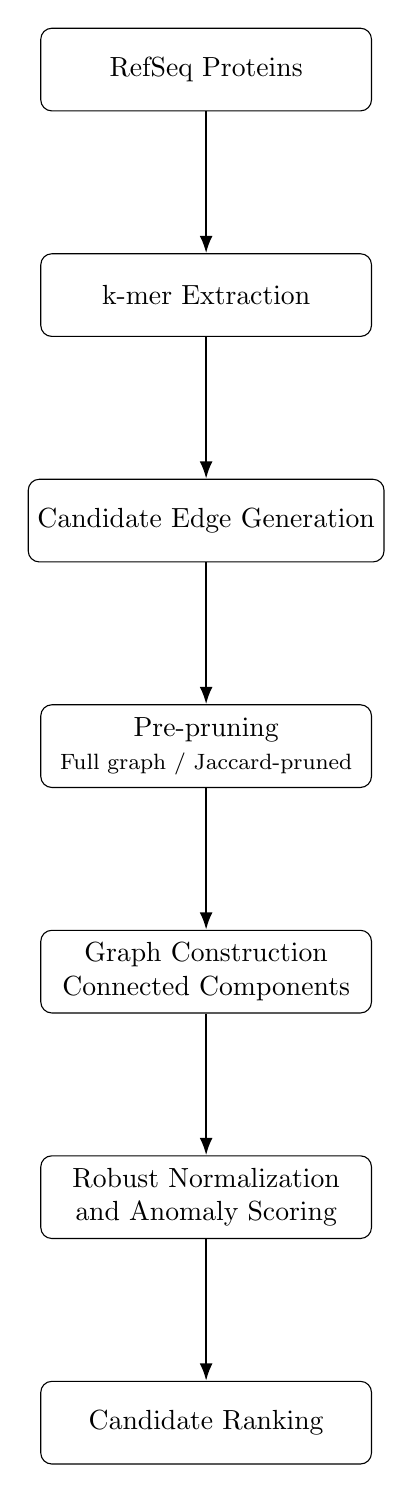
\begin{tikzpicture}[
    node distance=1.8cm,
    box/.style={draw, rectangle, rounded corners, align=center,
                minimum width=4.2cm, minimum height=1.05cm},
    arrow/.style={-{Latex[length=2.2mm]}, thick}
]
\node[box] (data) {RefSeq Proteins};
\node[box, below=of data] (kmers) {k-mer Extraction};
\node[box, below=of kmers] (cand) {Candidate Edge Generation};
\node[box, below=of cand] (prune) {Pre-pruning\\{\footnotesize Full graph / Jaccard-pruned}};
\node[box, below=of prune] (graph) {Graph Construction\\Connected Components};
\node[box, below=of graph] (score) {Robust Normalization\\and Anomaly Scoring};
\node[box, below=of score] (rank) {Candidate Ranking};

\draw[arrow] (data) -- (kmers);
\draw[arrow] (kmers) -- (cand);
\draw[arrow] (cand) -- (prune);
\draw[arrow] (prune) -- (graph);
\draw[arrow] (graph) -- (score);
\draw[arrow] (score) -- (rank);
\end{tikzpicture}
\caption{Overview of the HGT candidate detection pipeline. Protein sequences are represented using k-mers to
generate cross-species similarity candidates. Pre-pruning controls graph density by retaining high-confidence
edges, after which robust normalization and graph-based anomaly scoring are applied to identify candidate
HGT-related proteins.}
\label{fig:pipeline_overview}
\end{figure}

\subsection{Similarity Candidate Generation}
An all-vs-all protein comparison is computationally infeasible at this scale. Instead, proteins were represented as sets of distinct k-mers ($k=6$), encoded as collision-free base-20 integers over the canonical amino acid alphabet. Alignment-free sequence comparison based on k-mer statistics has been widely used for scalable genomic analysis \cite{Sims2009,Haubold2014}.  k-mers containing non-canonical residues were skipped.

The choice k = 6 reflects a practical compromise between sensitivity and specificity: smaller k increases spurious overlap due to random matches, while larger k reduces sensitivity to moderately diverged homologs and increases sparsity. Systematic exploration of k values remains future work.

Candidate protein pairs were proposed only if they shared a minimum number of distinct k-mers. Highly frequent k-mers were excluded to suppress non-informative overlaps, and only cross-species pairs were considered, as intra-species similarity is expected and not informative for HGT detection. To further bound complexity, candidate lists were capped to a fixed number of top matches per protein.

We compute exact Jaccard similarity over k-mer sets for candidate pairs. While sketching approaches such as MinHash can approximate Jaccard similarity and further reduce runtime and
memory for massive collections, exact Jaccard provides deterministic scores and was sufficient
at the current dataset scale. Extending the pipeline to MinHash-style sketches is straightforward and would enable scaling to substantially larger protein databases \cite{Broder1997,Ondov2016}.

\subsection{Graph Construction and Pruning}
Candidate pairs were assembled into an undirected, weighted similarity graph, with edges weighted by Jaccard similarity of k-mer sets. To obtain interpretable structure, multiple pruning steps were applied. Similarities were normalized within species pairs by retaining only the strongest edges relative to species-pair baselines. Per-node degree was capped by retaining only top-scoring edges per protein, preventing highly conserved proteins from dominating graph structure. Optional taxonomic distance filters were available to suppress edges likely reflecting vertical inheritance (homologous similarity between closely related taxa), thereby focusing the graph on taxonomically unexpected similarity more consistent with HGT.

These steps reduced the graph from approximately $9\times 10^5$ candidate edges to 92{,}790 edges, producing a sparse graph suitable for structural analysis.

\subsection{Graph-Based Anomaly Scoring}

HGT detection was framed as an anomaly detection problem. 
For most species pairs, cross-species protein similarity reflects background evolutionary conservation. 
Proteins involved in horizontal transfer are therefore expected to exhibit unusually strong similarity relative to their species-pair baseline.

Isolated anomalous edges, however, are insufficient evidence for transfer. 
True HGT events frequently involve multiple proteins, shared mobile elements, or functional modules, 
producing structured patterns of cross-species connectivity \cite{Frost2005,Ochman2000}. 
Representing similarities as a graph enables detection of such structure: proteins can be evaluated not only by the magnitude of individual anomalous similarities, but also by their position within mixed-species components, their potential bridge-like role between taxa, and the concentration of anomalous edges in their neighborhood.

To normalize similarity scores across heterogeneous species pairs, we computed robust $z$-scores using the median and median absolute deviation (MAD), a scale estimator resistant to heavy-tailed distributions \cite{Rousseeuw1993} arising from conserved protein families.

Connected components of the pruned graph were analyzed at multiple scales. 
At the component level, we quantified taxonomic mixing using the number of represented species and the Shannon entropy of the node species distribution, normalized by $\log k$, where $k$ is the number of species present (yielding values in $[0,1]$). 
We further measured anomaly concentration as the fraction of edges in the component whose robust $z$-score exceeded a fixed threshold.

At the node level, proteins were characterized by both local anomaly evidence (maximum and top-$k$ mean robust $z$-scores of incident edges) and structural role. 
Structural features included cross-species degree, normalized entropy of neighbor species labels, participation coefficient (quantifying how evenly a protein’s edges are distributed across taxa \cite{Guimera2005}), clustering coefficient (measuring the density of interconnections among a protein’s neighbors), and betweenness centrality computed on the high-anomaly subgraph.

Proteins were ranked using a component-aware scoring framework with explicit threshold-based gates. 
Candidates were required to belong to sufficiently large and taxonomically mixed components, 
to exhibit non-trivial anomalous similarity (robust $z$-scores above a minimum threshold), 
and to satisfy structural criteria such as minimum cross-species connectivity or bridge-like topology. 
Proteins failing these hard filters were assigned a score of zero.

For an eligible protein $u$ in component $C_u$, the final ranking score was defined multiplicatively as
\begin{equation}
S(u) = \Phi(C_u)\, A(u)\, T(u),
\end{equation}
where $\Phi(C_u)$ captures component-level context, 
$A(u)$ reflects local anomaly strength, 
and $T(u)$ summarizes graph-topological structure.

The context term $\Phi(C_u)$ increases with normalized species entropy and the concentration of high-surprise edges within $C_u$. 
The anomaly term $A(u)$ aggregates robust, species-pair–normalized similarity scores incident to $u$. 
The structural term $T(u)$ encodes cross-species connectivity and bridge-like centrality.

To stabilize scale differences across heterogeneous components, aggregation was performed in log-space:
\begin{equation}
\log S(u) = \log \Phi(C_u) + \log A(u) + \log T(u),
\end{equation}
so that high scores arise only when strong anomalous similarity co-occurs with substantial taxonomic mixing and informative graph structure.

\subsection{Implementation and Reproducibility}

All code and intermediate artifacts required to reproduce the reported results are available in the accompanying repository. We report here the exact parameterization used in each pipeline stage.

\textbf{Candidate generation.}
Proteins shorter than 50 amino acids were excluded. Sequences were represented as sets of distinct encoded $k$-mers with $k=6$. An inverted index was constructed, excluding high-frequency $k$-mers with posting list size $>100$. Candidate protein pairs were required to share at least 6 distinct $k$-mers, and for each protein we retained the top 10 cross-species matches by shared $k$-mer count. Only cross-species pairs were considered.

\textbf{Graph pre-pruning.}
Within each unordered species pair, edges were filtered to retain only the top 10\% by Jaccard similarity (0.9 quantile threshold). Per-node degree was capped at 20 by retaining the strongest incident edges per protein. Taxonomic filtering excluded edges with distance $<2$, and retained edges only if taxonomic distance $\le 4$ and Jaccard similarity $\ge 0.1$.

\textbf{Robust normalization and scoring.}
Robust $z$-scores were computed per species pair using the median and MAD ($1.4826 \cdot \mathrm{MAD} + 10^{-9}$), requiring at least 30 edges per species pair. Edges with $z \ge 3.0$ were considered high-surprise. Candidate ranking applied hard gates requiring component size $\ge 10$, normalized species entropy $\ge 0.75$, node degree $\ge 4$, mean top-5 incident surprise $\ge 2.0$, and either connectivity to at least three distinct species or non-zero betweenness centrality in the high-surprise subgraph.


% =========================
% 4. Results
% =========================
\section{Results}

\subsection{Graph scale and impact of pre-pruning}

\begin{figure}[!t]
    \centering
    
\includegraphics[width=0.5\linewidth]{z_score_distribution.png}
    \caption{Distribution of MAD-based Z-score for all protein-protein edges, plotted in logarithmic y-axis. The background distribution (grey) represents the global set of 911,306 edges, which clusters near the median (Z~0), reflecting expected evolutionary divergence. The dashed black line is the statistical significance threshold (Z=3). Edges connected to the final HGT candidates (red) are localized to the right tail of the distribution.}
    \label{fig:zscoredist}
\end{figure}

To assess the impact of pre-pruning on structural interpretability, we compare the Jaccard-pruned similarity graph, used for all structural analyses below, with the full candidate graph derived from the same RefSeq protein collection.

The full candidate graph contains 911{,}306 cross-species edges over 214{,}136 proteins. After Jaccard-based pre-pruning, the working graph contains 92{,}790 edges over 37{,}421 proteins and decomposes into 5{,}262 connected components.

Component size in the pruned graph is highly skewed (median = 4 nodes; 95th percentile = 20; maximum = 107), indicating that most similarity structure is localized and small-scale. Taxonomic mixing is similarly limited: the median component spans only two species, and only 18.5\% of components contain five or more species.

Anomalous similarity is globally sparse but concentrated in a small minority of components. The median fraction of high-$z$ edges per component is 0, and only 3.9\% of components exhibit substantial anomaly concentration ($high\_z\_frac > 0.3$). Thus, components combining extensive taxonomic mixing with concentrated high-surprise similarity represent rare structural regimes within the graph.

Across all 37{,}421 proteins in the pruned graph, only 5.9\% satisfy the structural and statistical gating criteria and receive a non-zero score, indicating strong selectivity of the ranking framework.

\subsection{Structural regimes in the Jaccard-pruned graph}

We next examine connected components that combine high anomaly concentration with broad taxonomic mixing, as identified by the scoring framework. Across these high-scoring components, anomalous edges form coherent structural backbones rather than appearing as isolated outliers. Candidate proteins frequently occupy bridge-like positions connecting distant taxa, consistent
with structured multi-species exchange patterns.


\subsubsection{Broad multi-taxa exchange module (Component 5)}

\begin{figure}[!t]
  \centering
  \includegraphics[height=0.45\textheight]{figures/component_5.png}
  \caption{Component 5: Broad multi-taxa exchange module. Nodes represent proteins and edges represent
  cross-species similarity. Node size reflects candidate score, and highlighted edges correspond to
  high-surprise similarities relative to species-pair baselines.}
  \label{fig:component5}
\end{figure}

Component 5 comprises 97 proteins connected by 632 edges (density = 0.136), spanning 50 species with near-maximal normalized entropy (H$_{\mathrm{norm}}$ = 0.998) and a high anomaly concentration (high\_z\_frac = 0.60; max robust $z$ = 19.81) (Figure~\ref{fig:component5}).

Despite dense background connectivity, a large fraction of edges exhibits high surprise, including multiple extreme outliers connecting taxonomically distant organisms. High-scoring proteins participate in multiple cross-species interactions and are distributed throughout the component, indicating a shared exchange module rather than a single anomalous pair. This organization is consistent with repeated horizontal transfer or shared mobile gene pools that generate coherent multi-species similarity structure.

\subsubsection{Chained cross-species transfer structure (Component 8)}

\begin{figure}[!t]
  \centering
  \includegraphics[height=0.45\textheight]{figures/component_8.png}
  \caption{Component 8: Chained cross-species connectivity. Compact sub-clusters are linked by a small number
  of high-surprise edges, producing elongated paths across distant taxa.}
  \label{fig:component8}
\end{figure}

Component 8 comprises 95 proteins connected by 589 edges (density = 0.13), spanning 49 species with near-maximal normalized entropy (H$_{\mathrm{norm}}$ = 0.998) and high anomaly concentration (high\_z\_frac = 0.47) (Figure~\ref{fig:component8}).

The component contains compact subclusters connected by a limited number of high-surprise edges, producing elongated chains linking distant taxa. Such chained connectivity suggests stepwise propagation or modular transfer patterns in which related genetic material appears across multiple lineages through intermediate connections, rather than concentrating into a single hub.

\subsubsection{Localized high-confidence bridges (Component 32)}

\begin{figure}[t]
  \centering
  \includegraphics[width=\linewidth]{figures/component_32.png}
  \caption{Component 32: Localized high-confidence bridges. Two coherent regions are connected by a small
  number of strong cross-species edges, with anomalous signal concentrated in the bridges.}
  \label{fig:component32}
\end{figure}

Component 32 contains 71 proteins across 31 species(H$_{\mathrm{norm}}$ = 0.958) but exhibits low anomaly concentration (high\_z\_frac = 0.063), representing a mixed yet largely non-anomalous regime (Figure~\ref{fig:component32}).

The anomalous signal is concentrated in a small number of bridging edges, while the remaining connectivity reflects ordinary similarity context. This structure is consistent with localized transfer-like events linking otherwise unrelated taxa.

\subsection{Comparison with the full candidate graph}

Applying the same normalization and structural scoring to the full candidate graph yields substantially denser connectivity, with many additional proteins and edges that obscure component boundaries. Although high-surprise edges and mixed-species hotspots remain detectable, large components become less separable and qualitative interpretation is significantly reduced. This contrast supports pre-pruning as a practical requirement for extracting interpretable HGT-like modules at scale.

\subsection{Score distribution and selectivity}

Among the top 200 ranked proteins, the median score was 5.9 (IQR: 4.47–8.17), with the 95th percentile at 12.74 and a maximum of 18.76. These values represent the upper tail of the scoring distribution within the 5.9\% of proteins that passed gating, reinforcing that high-ranking candidates reflect extreme combinations of anomalous similarity, taxonomic mixing,
and structural bridging evidence.

Implementation details, configuration parameters, and full reproducibility artifacts for both pruning regimes are available in the accompanying GitHub repository~\cite{HGTRepo2026}.

\FloatBarrier

% =========================
% 5. Discussion
% =========================
\section{Discussion}
\label{sec:discussion}

Our method is intended as a scalable hypothesis-generation framework rather than a definitive test for horizontal gene transfer. By replacing alignment and phylogenetic reconstruction with species-aware normalization and graph-structural analysis, we trade resolution for scalability, prioritizing candidates for downstream validation rather than directly confirming transfer events.

Several design choices reflect explicit trade-offs. Restricting candidate generation using
$k=6$, requiring at least six shared $k$-mers, limiting posting lists to size 100, and retaining
only the top 10 cross-species matches per protein aggressively suppresses conserved motifs and
ubiquitous housekeeping genes. While this substantially reduces false positives arising from
generic conservation, it may also exclude true transfer events involving highly conserved or
short protein domains. Similarly, per-species-pair percentile pruning (top 10\%) and degree
capping (top 20 edges per node) improve structural interpretability but introduce heuristic
thresholds that may affect sensitivity.

The robust $z$-score normalization mitigates heterogeneity across species pairs, yet its
effectiveness depends on sufficient edge counts per pair (minimum 30). Rare species pairs with
few observations may therefore yield unstable baselines. In addition, anomaly thresholds
(e.g., $z \ge 3$) emphasize extreme deviations and may bias the ranking toward dramatic
cross-species similarities while overlooking subtler but biologically meaningful transfers.

False positives remain possible in cases of convergent evolution, shared ancient homologous, or
unmodeled taxonomic structure. Conversely, false negatives may arise when transfer events occur
between closely related taxa that were filtered by taxonomic distance thresholds, or when
post-transfer divergence reduces $k$-mer overlap below detection limits.

Despite these limitations, the consistency of signal across edge-level anomaly, node-level
connectivity, and component-level taxonomic mixing suggests that high-ranking candidates are
not artifacts of a single heuristic. Instead, they represent multi-scale structural deviations from
expected background similarity.

Future validation should integrate orthogonal genomic evidence, including synteny conservation,
plasmid or genomic island association, and phylogenetic incongruence analysis. Sensitivity
analysis over $k$, pruning percentiles, and anomaly thresholds would further clarify robustness
and support scaling to larger protein collections.

% =========================
% 6. Conclusion
% =========================
\section{Conclusion}

We presented a scalable, alignment-free framework for large-scale HGT candidate detection based on species-pair–aware normalization and sparse similarity graphs. By combining robust statistical calibration with graph-structural features and explicit gating criteria, the method selectively reduces large protein collections to a compact, interpretable set of high-priority candidates suitable for downstream phylogenetic and genomic validation.

% =========================
% 7. Work Distribution
% =========================
\section*{Work Distribution}
\begin{table}[h]
\centering
\begin{tabular}{lccccc}
\hline
Task & Or & Noam K. & Roee & Dor & Noam K. \\
\hline
Data acquisition and preprocessing &  &  &  &  &  \\
Graph design and methodology &  &  &  &  &  \\
Implementation and optimization &  &  &  &  &  \\
Statistical analysis &  &  &  &  &  \\
Visualization and figures &  &  &  &  &  \\
Writing – Methods &  &  &  &  &  \\
Writing – Results &  &  &  &  &  \\
Writing – Discussion &  &  &  &  &  \\
\hline
\end{tabular}
\caption{Division of responsibilities among team members.}
\end{table}

\appendix
\section{Reproduction Recipe}
\begin{verbatim}
# Candidate generation
python kmer_candidates_from_faa.py \
  --manifest data/out_refseq/manifest.tsv \
  --downloads_dir data/out_refseq/downloads \
  --out data/out_refseq/candidates.tsv \
  --k 6 --min_len 50 --max_postings 100 \
  --min_shared 6 --top_m 10 --cross_species_only

# Graph pruning (parameters hard-coded in script)
python graph_pruning.py

# Graph scoring and ranking
python graph_hgt_pipeline.py --in_edges pruned_edges.tsv --out_dir outputs/
\end{verbatim}

% =========================
% References
% =========================
\bibliographystyle{unsrt}
\bibliography{references}

\end{document}
